\documentclass[systemskiss/skiss.tex]{subfiles}

\begin{document}
\section{Sensormodul}
<<<<<<< HEAD
Sensormodulen innehåller alla de sensorer som bilen behöver för att kunna mäta avstånd i sin omgivning. Den är direkt kopplad till kommunikationsmodulen via en databuss.
=======
Sensormodulen innehåller alla de sensorer som bilen behöver för att kunna mäta avstånd i sin omgivning. Den är d<irekt kopplad till kommunikationsmodulen via en databuss.
>>>>>>> 04d2f39596c86215d9343d345750e4e73c36afa1
\subsection{Översiktlig beskrivning av modulen}
\begin{figure}[h]
    \centering
    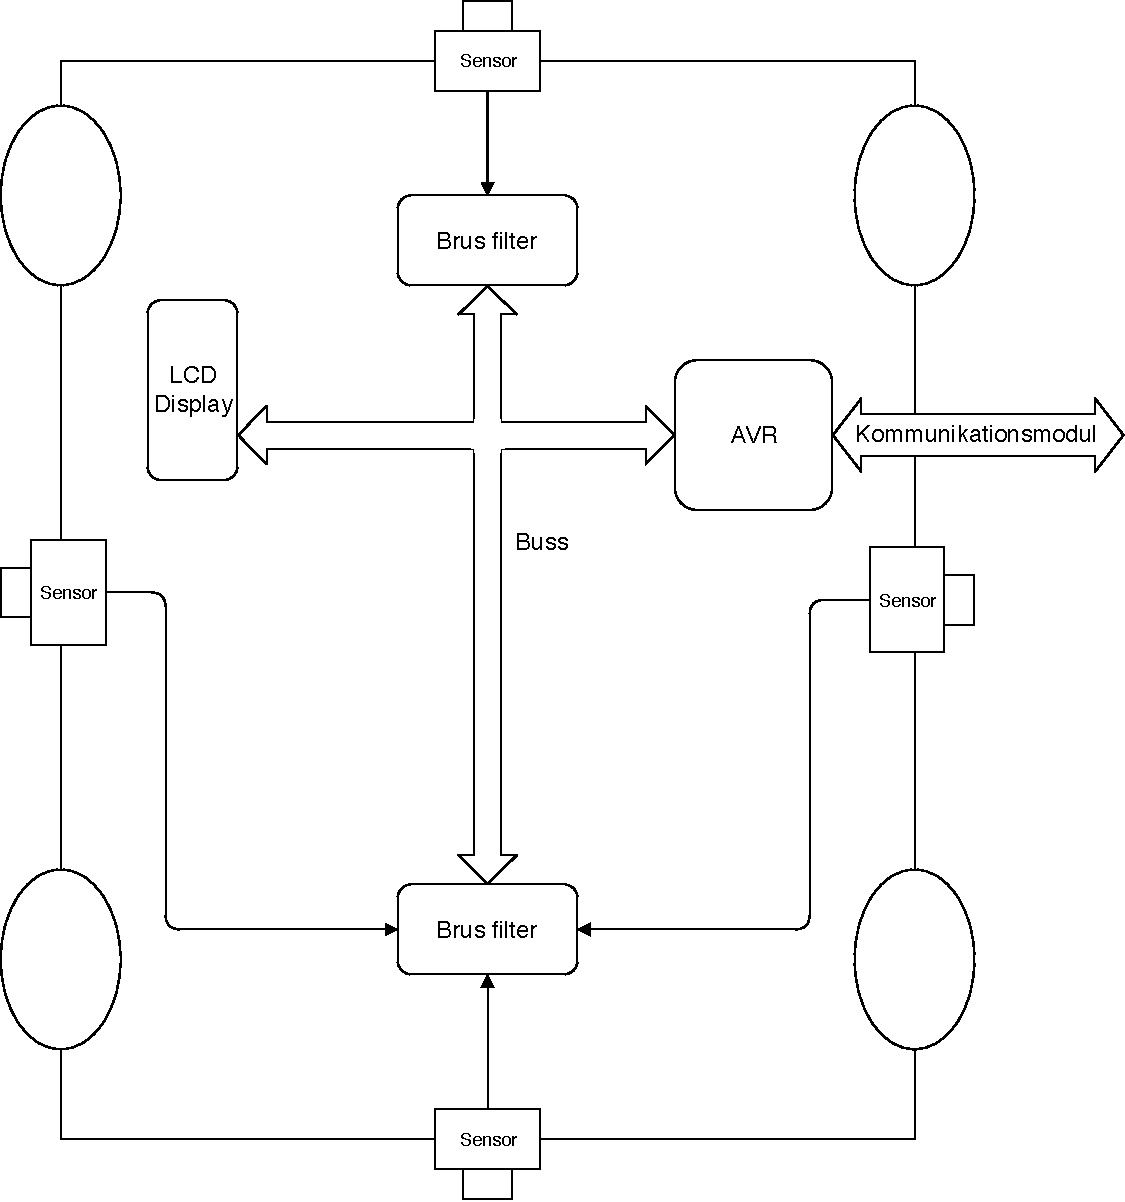
\includegraphics[width=0.6\linewidth]{systemskiss/figures/sensormodul.pdf}
    \caption{Övergripande bild över sensormodulen}
    \label{fig:sensorskiss}
\end{figure}

Sensorerna ska vara kopplade till olika brusfilter som gör signalern tydligare. När signalerna är filterade ska de skickas via en databuss till modulens processor. Databussen ska även vara kopplad till en LCD skärm där värdena ska visas för att förenkla felsökning av modulen. Modulen ska ha en direkt koppling till kommunikationsmodulen via en databuss. Figur \ref{fig:sensorskiss} visar en grov bild över hur modulen ska se ut.


\end{document}

